\documentclass[tikz,border=4pt]{standalone}
\usepackage{tikz}
\usetikzlibrary{arrows.meta,positioning,shapes.geometric}

\begin{document}
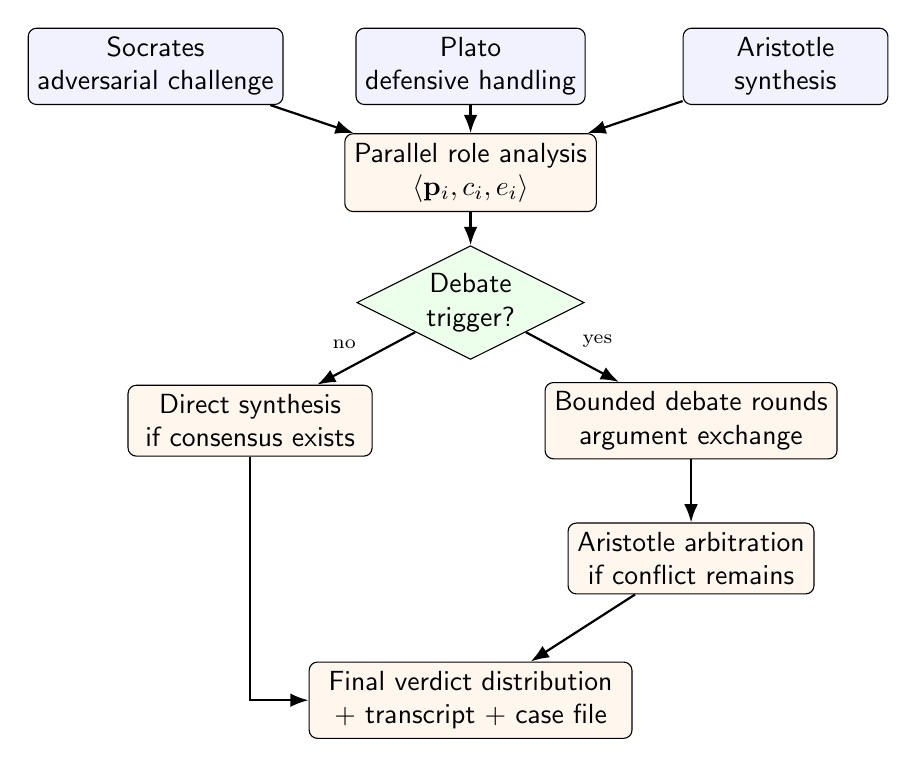
\begin{tikzpicture}[
  font=\sffamily,
  role/.style={draw, rounded corners=3pt, align=center, minimum width=2.6cm, minimum height=0.95cm, fill=blue!5},
  proc/.style={draw, rounded corners=3pt, align=center, minimum width=3.1cm, minimum height=0.9cm, fill=orange!7},
  decision/.style={diamond, draw, aspect=2.0, align=center, fill=green!8, inner sep=1.4pt},
  arrow/.style={-Latex, thick}
]

\node[role] (soc) at (0,2.3) {Socrates\\adversarial challenge};
\node[role] (pla) at (4,2.3) {Plato\\defensive handling};
\node[role] (ari) at (8,2.3) {Aristotle\\synthesis};

\node[proc] (parallel) at (4,0.95) {Parallel role analysis\\$\langle \mathbf{p}_i, c_i, e_i \rangle$};
\node[decision] (trigger) at (4,-0.7) {Debate\\trigger?};
\node[proc] (consensus) at (1.2,-2.2) {Direct synthesis\\if consensus exists};
\node[proc] (debate) at (6.8,-2.2) {Bounded debate rounds\\argument exchange};
\node[proc] (arb) at (6.8,-3.95) {Aristotle arbitration\\if conflict remains};
\node[proc, minimum width=4.1cm] (final) at (4,-5.75) {Final verdict distribution\\+ transcript + case file};

\draw[arrow] (soc) -- (parallel);
\draw[arrow] (pla) -- (parallel);
\draw[arrow] (ari) -- (parallel);
\draw[arrow] (parallel) -- (trigger);
\draw[arrow] (trigger) -- node[above left, font=\scriptsize] {no} (consensus);
\draw[arrow] (trigger) -- node[above right, font=\scriptsize] {yes} (debate);
\draw[arrow] (debate) -- (arb);
\draw[arrow] (consensus) |- (final.west);
\draw[arrow] (arb) -- (final);

\end{tikzpicture}
\end{document}
